%\documentclass[UTF8]{ctexart} % use larger type; default would be 10pt
\documentclass[a4paper]{article}
\usepackage{xeCJK}
%\usepackage[utf8]{inputenc} % set input encoding (not needed with XeLaTeX)

%%% Examples of Article customizations
% These packages are optional, depending whether you want the features they provide.
% See the LaTeX Companion or other references for full information.

%%% PAGE DIMENSIONS
\usepackage{geometry} % to change the page dimensions
\geometry{a4paper} % or letterpaper (US) or a5paper or....
\geometry{margin=1in} % for example, change the margins to 2 inches all round
% \geometry{landscape} % set up the page for landscape
%   read geometry.pdf for detailed page layout information

\usepackage{graphicx} % support the \includegraphics command and options

% \usepackage[parfill]{parskip} % Activate to begin paragraphs with an empty line rather than an indent

%%% PACKAGES
\usepackage{booktabs} % for much better looking tables
\usepackage{array} % for better arrays (eg matrices) in maths
\usepackage{paralist} % very flexible & customisable lists (eg. enumerate/itemize, etc.)
\usepackage{verbatim} % adds environment for commenting out blocks of text & for better verbatim
\usepackage{subfig} % make it possible to include more than one captioned figure/table in a single float
% These packages are all incorporated in the memoir class to one degree or another...

%%% HEADERS & FOOTERS
\usepackage{fancyhdr} % This should be set AFTER setting up the page geometry
\pagestyle{fancy} % options: empty , plain , fancy
\renewcommand{\headrulewidth}{0pt} % customise the layout...
\lhead{}\chead{}\rhead{}
\lfoot{}\cfoot{\thepage}\rfoot{}

%%% SECTION TITLE APPEARANCE
\usepackage{sectsty}
\allsectionsfont{\sffamily\mdseries\upshape} % (See the fntguide.pdf for font help)
% (This matches ConTeXt defaults)

%%% ToC (table of contents) APPEARANCE
\usepackage[nottoc,notlof,notlot]{tocbibind} % Put the bibliography in the ToC
\usepackage[titles,subfigure]{tocloft} % Alter the style of the Table of Contents
\renewcommand{\cftsecfont}{\rmfamily\mdseries\upshape}
\renewcommand{\cftsecpagefont}{\rmfamily\mdseries\upshape} % No bold!

%%% END Article customizations

%%% The "real" document content comes below...

\setlength{\parindent}{0pt}
\usepackage{physics}
\usepackage{amsmath}
%\usepackage{symbols}
\usepackage{AMSFonts}
\usepackage{bm}
%\usepackage{eucal}
\usepackage{mathrsfs}
\usepackage{amssymb}
\usepackage{float}
\usepackage{multicol}
\usepackage{abstract}
\usepackage{empheq}
\usepackage{extarrows}
\usepackage{textcomp}
\usepackage{fontspec}
\usepackage{braket}
\usepackage{siunitx}
\sisetup{
	separate-uncertainty = true,
	inter-unit-product = \ensuremath{{}\cdot{}}
}
\usepackage{mhchem}
\usepackage{hyperref}
\hypersetup{
	colorlinks=true,
	linkcolor=black,
	filecolor=magenta,      
	urlcolor=cyan,
}

\DeclareMathOperator{\p}{\prime}
\DeclareMathOperator{\ti}{\times}
\DeclareMathOperator{\intinf}{\int_0^\infty}
\DeclareMathOperator{\intdinf}{\int_{-\infty}^\infty}
\DeclareMathOperator{\intzpi}{\int_0^\pi}
\DeclareMathOperator{\intztpi}{\int_0^{2\pi}}
\DeclareMathOperator{\sumninf}{\sum_{n=1}^{\infty}}
\DeclareMathOperator{\sumninfz}{\sum_{n=0}^\infty}
\DeclareMathOperator{\sumiinf}{\sum_{i=1}^{\infty}}
\DeclareMathOperator{\sumiinfz}{\sum_{i=0}^\infty}
\DeclareMathOperator{\sumkinf}{\sum_{k=1}^{\infty}}
\DeclareMathOperator{\sumkinfz}{\sum_{k=0}^\infty}
\DeclareMathOperator{\e}{\mathrm{e}}
\DeclareMathOperator{\I}{\mathrm{i}}
\DeclareMathOperator{\Arg}{\mathrm{Arg}}
\DeclareMathOperator{\ra}{\rightarrow}
\DeclareMathOperator{\llra}{\longleftrightarrow}
\DeclareMathOperator{\lra}{\longrightarrow}
\DeclareMathOperator{\dlra}{\Leftrightarrow}
\DeclareMathOperator{\dra}{\Rightarrow}
\newcommand{\bkk}[1]{\Braket{#1|#1}}
\newcommand{\bk}[2]{\Braket{#1|#2}}
\newcommand{\bkev}[2]{\Braket{#2|#1|#2}}



\DeclareMathOperator{\hV}{\hat{\vb{V}}}

\DeclareMathOperator{\hx}{\hat{\vb{x}}}
\DeclareMathOperator{\hy}{\hat{\vb{y}}}
\DeclareMathOperator{\hz}{\hat{\vb{z}}}

\DeclareMathOperator{\hA}{\hat{\vb{A}}}

\DeclareMathOperator{\hQ}{\hat{\vb{Q}}}
\DeclareMathOperator{\hI}{\hat{\vb{I}}}
\DeclareMathOperator{\psis}{\psi^\ast}
\DeclareMathOperator{\Psis}{\Psi^\ast}
\DeclareMathOperator{\hi}{\hat{\vb{i}}}
\DeclareMathOperator{\hj}{\hat{\vb{j}}}
\DeclareMathOperator{\hk}{\hat{\vb{k}}}
\DeclareMathOperator{\hr}{\hat{\vb{r}}}
\DeclareMathOperator{\hT}{\hat{\vb{T}}}
\DeclareMathOperator{\hH}{\hat{H}}
\DeclareMathOperator{\hh}{\hat{h}}               % helicity
\DeclareMathOperator{\hL}{\hat{\vb{L}}}
\DeclareMathOperator{\hp}{\hat{\vb{p}}}

\DeclareMathOperator{\ha}{\hat{\vb{a}}}
\DeclareMathOperator{\hS}{\hat{\vb{S}}}
\DeclareMathOperator{\hSigma}{\hat{\bm\Sigma}}
\DeclareMathOperator{\hJ}{\hat{\vb{J}}}
\DeclareMathOperator{\hP}{\hat{\vb{P}}}          % Parity
\DeclareMathOperator{\hC}{\hat{\vb{C}}} 
\DeclareMathOperator{\Tdv}{-\dfrac{\hbar^2}{2m}\dv[2]{x}}
\DeclareMathOperator{\Tna}{-\dfrac{\hbar^2}{2m}\nabla^2}
\DeclareMathOperator{\vna}{\vnabla}
\DeclareMathOperator{\nna}{\nabla^2}
\newcommand{\naCarExpd}[1]{\pdv[2]{#1}{x} + \pdv[2]{#1}{y} + \pdv[2]{#1}{z}}
\newcommand{\naCyl}{\qty[\dfrac{1}{\rho}\pdv{\rho}\qty(\rho\pdv{\rho}) + \dfrac{1}{\rho^2}\pdv[2]{\phi} + \pdv[2]{z}]}

%\DeclareMathOperator{\g#0}{\gamma^0}
%\DeclareMathOperator{\g1}{\gamma^1}
%\DeclareMathOperator{\g2}{\gamma^2}
%\DeclareMathOperator{\g3}{\gamma^3}
%\DeclareMathOperator{\g5}{\gamma^5}
\newcommand{\g}[1]{\gamma^{#1}}
\DeclareMathOperator{\gmuu}{\gamma^\mu}
\DeclareMathOperator{\gmud}{\gamma_\mu}
%\newcommand{\G}[2]{g^{#1#2}}

\newcommand{\subsbul}{\subsection*{$ \bullet $}}
\newcommand{\ex}[1]{\paragraph{12-#1}}
\newcommand{\subex}[1]{\subparagraph{#1}}
\newcommand{\dis}{\displaystyle}
\newcommand{\iden}{{\large \bm{1}}}
\newcommand{\qed}{$ \Square $}
\newcommand{\tPhi}{\tilde{\Phi} }

\numberwithin{equation}{section}
%\setcounter{secnumdepth}{4}
\setcounter{tocdepth}{4}
%\allowdisplaybreaks[4]

\usepackage{xcolor}
\definecolor{codegray}{gray}{0.9}
\newfontfamily\Consolas{Consolas}
\newcommand{\code}[1]{\colorbox{codegray}{{\Consolas#1}}}

\title{\textbf{Advanced Physical Chemistry II}\\HW}
\author{王石嵘
\vspace{5pt}\\
161240065\\
%Email: shirong\_wang@berkeley.edu
}
\date{\today} % Activate to display a given date or no date (if empty),
         % otherwise the current date is printed 

\begin{document}
% \boldmath

\maketitle

\tableofcontents

\newpage

\setcounter{section}{11}
\section{Group Theory: the Exploitation of Symmetry}
4, 12, 18, 24, 26, 31, 33, 34, 37, 40\\
\ex{4}
The symmetry elements of $ \ce{CH_4} $ is as follows. (each $ S_4 $ axis is coincident with $ C_2 $ axis)\footnote{The pictures are taken from \href{https://www.chemtube3d.com/methane-tetrahedral-symmetry-td/}{chemtube3d}.}
\begin{figure}[H]
	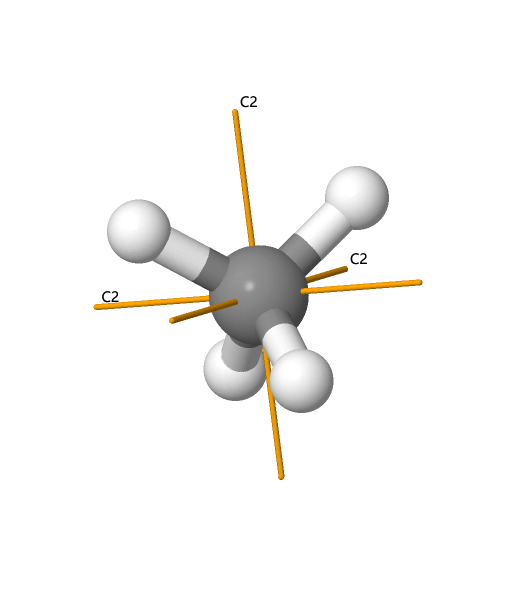
\includegraphics[width=0.3\linewidth]{methane_c2.png}
	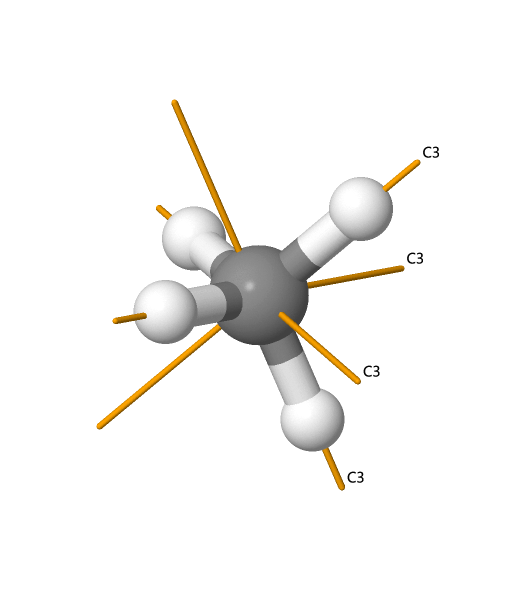
\includegraphics[width=0.3\linewidth]{methane_c3.png}
	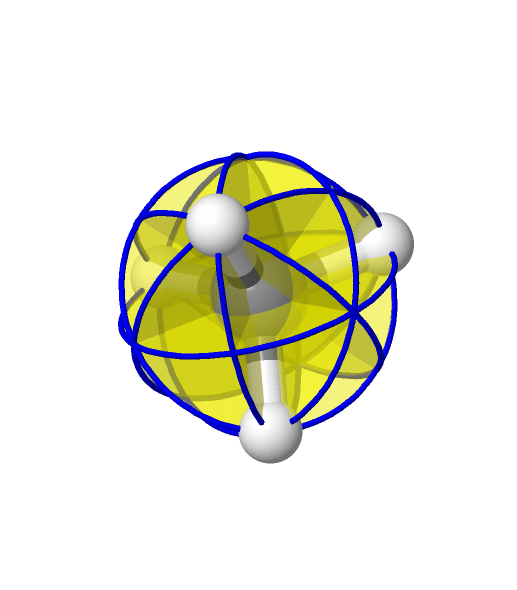
\includegraphics[width=0.37\linewidth]{methane_sigmad.png}
\end{figure}

\ex{12}
\begin{align}
C_3\sigma_v &= \sigma_v'\\
C_3\sigma_v'' &= \sigma_v
\end{align}

\ex{18}
For the irreducible representation of $ C_{3v} $,
\begin{align}
\hat{E}\mqty(u_x\\ u_y) &= \mqty(u_x\\ u_y)
\end{align}
Set the z-axis as $ C_3 $ axis, we have
\begin{equation}\label{key}
\hat{C}_3\mqty(u_x\\ u_y) = \mqty(\cos\dfrac{-\pi}{3} & \sin\dfrac{-\pi}{3}\\ -\sin\dfrac{-\pi}{3} & \cos\dfrac{-\pi}{3})\mqty(u_x\\ u_y) 
= \mqty(-\dfrac{1}{2} & -\dfrac{\sqrt{3}}{2}\\ \dfrac{\sqrt{3}}{2} & -\dfrac{1}{2})\mqty(u_x\\ u_y)
\end{equation}
\begin{equation}\label{key}
\hat{C}_3^2\mqty(u_x\\ u_y) = \mqty(\cos\dfrac{-2\pi}{3} & \sin\dfrac{-2\pi}{3}\\ -\sin\dfrac{-2\pi}{3} & \cos\dfrac{-2\pi}{3})\mqty(u_x\\ u_y) 
= \mqty(-\dfrac{1}{2} & \dfrac{\sqrt{3}}{2}\\ -\dfrac{\sqrt{3}}{2} & -\dfrac{1}{2})\mqty(u_x\\ u_y)
\end{equation}
Set the x-axis on $ \sigma_v $, we have
\begin{equation}\label{key}
\left\{\mqty{\hat\sigma_v u_x &= u_x\\ \hat\sigma_v u_y &= -u_y} \right.
\dra \hat\sigma_v\mqty(u_x\\ u_y) = \mqty(1 & 0\\ 0 & -1)\mqty(u_x\\ u_y)
\end{equation}
Similarly, we get
\begin{align}
\hat\sigma_v'\mqty(u_x\\ u_y) &= \mqty(-\dfrac{1}{2} & \dfrac{\sqrt{3}}{2}\\ \dfrac{\sqrt{3}}{2} & \dfrac{1}{2})\mqty(u_x\\ u_y)\\
\hat\sigma_v''\mqty(u_x\\ u_y) &= \mqty(-\dfrac{1}{2} & -\dfrac{\sqrt{3}}{2}\\ -\dfrac{\sqrt{3}}{2} & \dfrac{1}{2})\mqty(u_x\\ u_y)
\end{align}
Thus, $ (u_x, u_y) $ forms a joint basis for the irreducible representation of $ C_{3v} $.

\ex{24}
No, because $ 2p_{zN} $ and $ 1s_{H_A} + 1s_{H_B} + 1s_{H_C} $ both belongs to $ A_1 $.

\ex{26}
\subex{$ \bullet $}
\begin{align}\label{key}
\dfrac{\sqrt{12}}{6}(2\phi_4 - \phi_3) &= \dfrac{\sqrt{12}}{6}\qty[2\dfrac{1}{\sqrt{12}}\qty(\psi_1 + 2\psi_2 + \psi_3 - \psi_4 - 2\psi_5 - \psi_6) - \dfrac{1}{\sqrt{12}}\qty(2\psi_1 + \psi_2 - \psi_3 - 2\psi_4 - \psi_5 + \psi_6)] \notag\\
&= \dfrac{1}{6}(0 + 3\psi_2 + 3\psi_3 + 0 -3\psi_5 - 3\psi_6)\notag\\
&= \dfrac{1}{2}(\psi_2 + \psi_3 - \psi_5 - \psi_6) \notag\\
&= \phi_4'
\end{align}
\subex{$ \bullet $}
\begin{align}
\Braket{\phi_4' | \phi_4'} &= \dfrac{1}{3}\Braket{2\phi_4 - \phi_3 | 2\phi_4 - \phi_3} \notag\\
&= \dfrac{1}{3}(4 + 1 - 4\Braket{\phi_4|\phi_3})
\end{align}
while
\begin{align}\label{key}
\Braket{\phi_4|\phi_3} &= \dfrac{1}{12}\Braket{\psi_1 + 2\psi_2 + \psi_3 - \psi_4 - 2\psi_5 - \psi_6 | 2\psi_1 + \psi_2 - \psi_3 - 2\psi_4 - \psi_5 + \psi_6} \notag\\
&= \dfrac{1}{12}(2 + 2 - 1 + 2 + 2 - 1) \notag\\
&= \dfrac{1}{2}
\end{align}
thus
\begin{equation}\label{key}
\Braket{\phi_4' | \phi_4'} = \dfrac{1}{3}\qty(5 - 4\cross\dfrac{1}{2}) = 1
\end{equation}
$ \therefore $ $ \phi_4' $ is normalized.
\subex{$ \bullet $}
\begin{align}
S_{33}' &= S_{44}' = 1\\
S_{34}' &= S_{43}' = \dfrac{\sqrt{12}}{6}\Braket{\phi_3 | 2\phi_4 - \phi_3} = 0\\
H_{33}' &= \Braket{\phi_3 | \hH | \phi_3} = \dfrac{1}{12}(12\alpha + 12\beta) = \alpha+\beta\\
H_{44}' &= \Braket{\phi_4 | \hH | \phi_4} = \dfrac{1}{4}(4\alpha + 4\beta) = \alpha+\beta\\
H_{34}' &= H_{43}' = \Braket{\phi_3 | \hH | \phi_4} = \dfrac{1}{2\sqrt{12}}(0 + 0) = 0
\end{align}
thus
\begin{equation}\label{key}
\mqty|\alpha + \beta - E & 0\\ 0 & \alpha + \beta - E| = 0 \;\dra\; E = \alpha+\beta 
\end{equation}
\ex{31}
\subex{$ \bullet $}
Since $ H_{ii} = \alpha $, $ H_{12} = H_{23} = \beta $, $ S_{ij} = \delta_{ij} $, we have
\begin{equation}\label{key}
\mqty|\alpha - E & \beta & 0 \\ \beta & \alpha-E & \beta\\ 0 & \beta & \alpha-E| = \beta^3\mqty|x & 1 & 0\\ 1 & x& 1\\ 0 & 1 & x| = 0
\end{equation}
thus
\begin{equation}\label{key}
x^3 - 2x = 0 \;\dra\; x= 0, \pm\sqrt{2}
\end{equation}
\subex{$ \bullet $}
$ C_{2v} $ group has 4 operators, $ \hat{E}, \hat{C}_2, \hat\sigma_v, \hat\sigma_v' $.
%% How to distinguish sigma_v and sigma_v'?
\begin{align}
\hat{E}\mqty(\psi_1\\\psi_2\\\psi_3) &= \mqty(1 & 0 & 0\\ 0 & 1 & 0\\ 0 & 0 & 1) \mqty(\psi_1\\\psi_2\\\psi_3) \\
\hat{C}_2\mqty(\psi_1\\\psi_2\\\psi_3) &= \mqty(0 & 0 & -1\\ 0 & -1 & 0\\ -1 & 0 & 0) \mqty(\psi_1\\\psi_2\\\psi_3) \\
\hat\sigma_v\mqty(\psi_1\\\psi_2\\\psi_3) &= \mqty(0 & 0 & 1\\ 0 & 1 & 0\\ 1 & 0 & 0) \mqty(\psi_1\\\psi_2\\\psi_3) \\
\hat\sigma_v'\mqty(\psi_1\\\psi_2\\\psi_3) &= \mqty(-1 & 0 & 0\\ 0 & -1 & 0\\ 0 & 0 & -1) \mqty(\psi_1\\\psi_2\\\psi_3) 
\end{align}
Collect the traces of the matrices above, we get
\begin{equation}\label{key}
 \Gamma = \mqty{3 & -1 & 1 & -3} 
\end{equation}
\subex{$ \bullet $}
\begin{align}
a_{A_1} &= \dfrac{1}{4}[3\cross 1 + (-1)\cross 1 + 1\cross 1 + (-3)\cross 1] = 0\\
a_{A_2} &= \dfrac{1}{4}[3\cross 1 + (-1)\cross 1 + 1\cross (-1) + (-3)\cross (-1)] = 1\\
a_{B_1} &= \dfrac{1}{4}[3\cross 1 + (-1)\cross (-1) + 1\cross 1 + (-3)\cross (-1)] = 2\\
a_{B_2} &= \dfrac{1}{4}[3\cross 1 + (-1)\cross (-1) + 1\cross (-1) + (-3)\cross 1] = 0
\end{align}
thus
\begin{equation}\label{key}
\Gamma = A_2 + 2B_2
\end{equation}
which means the secular determinant can be written as the combination of a 1D block and a 2D block.
\subex{$ \bullet $}
Now we generate the symmetric orbitals
\begin{align}
\hP_{A_2}\psi_1 &= \dfrac{1}{4}(\psi_1 - \psi_3 - \psi_3 + \psi_1) = \dfrac{1}{2}(\psi_1 - \psi_3)\\
\hP_{B_1}\psi_1 &= \dfrac{2}{4}(\psi_1 + \psi_3 + \psi_3 + \psi_1) = \psi_1 + \psi_3\\
\hP_{B_1}\psi_2 &= \dfrac{2}{4}(\psi_2 + \psi_2 + \psi_2 + \psi_2) = 2\psi_2\\
\end{align}
After normalization,
\begin{align}
\phi_1 &= \dfrac{1}{\sqrt{2}}(\psi_1 - \psi_3)\\
\phi_2 &= \psi_2\\
\phi_3 &= \dfrac{1}{\sqrt{2}}(\psi_1 + \psi_3)\\
\end{align}
Thus,
\begin{equation}\label{key}
\mqty|\alpha - E & 0 & 0\\ 0 & \alpha - E & \sqrt{2}\beta\\ 0 & \sqrt{2}\beta & \alpha - E| 
= \beta^3\mqty|x & 0 & 0\\ 0 & x & \sqrt{2}\\ 0 & \sqrt{2} & x| = 0
\end{equation}
i.e.
\begin{equation}\label{key}
x(x^2 -2) = 0
\end{equation}
$ \therefore $
\begin{equation}\label{key}
E = 0, \pm\sqrt{2}
\end{equation}
i.e.
\begin{equation}\label{key}
E = \alpha, \alpha\pm\sqrt{2}\beta
\end{equation}

\ex{33}
\begin{enumerate}
	\item $ i=j=A_1 $
	\begin{equation}\label{key}
	\sum_R \Gamma_{A_1}(R)_{11}\Gamma_{A_1}(R)_{11} = 1 + 1 + 1 + 1 + 1 + 1 = \dfrac{6}{1}
	\end{equation}
	\item $ i=j=A_2 $
	\begin{equation}\label{key}
	\sum_R \Gamma_{A_2}(R)_{11}\Gamma_{A_2}(R)_{11} = 1 + 1 + 1 + 1 + 1 + 1 = \dfrac{6}{1}
	\end{equation}
	\item $ i=j=E $
	\begin{align}\label{key}
	\sum_R \Gamma_{E}(R)_{11}\Gamma_{E}(R)_{11} &= 1 + \dfrac{1}{4} + \dfrac{1}{4} + 1 + \dfrac{1}{4} + \dfrac{1}{4} = \dfrac{6}{2}\\
	\sum_R \Gamma_{E}(R)_{22}\Gamma_{E}(R)_{22} &= 1 + \dfrac{1}{4} + \dfrac{1}{4} + 1 + \dfrac{1}{4} + \dfrac{1}{4} = \dfrac{6}{2}\\
	\sum_R \Gamma_{E}(R)_{12}\Gamma_{E}(R)_{12} &= 0 + \dfrac{3}{4} + \dfrac{3}{4} + 0 + \dfrac{3}{4} + \dfrac{3}{4} = \dfrac{6}{2}\\
	\sum_R \Gamma_{E}(R)_{11}\Gamma_{E}(R)_{12} &= 0 + \dfrac{\sqrt{3}}{4} -\dfrac{\sqrt{3}}{4} + 0 - \dfrac{\sqrt{3}}{4} + \dfrac{\sqrt{3}}{4} = 0\\
	\sum_R \Gamma_{E}(R)_{11}\Gamma_{E}(R)_{22} &= 1 + \dfrac{1}{4} + \dfrac{1}{4} - 1 - \dfrac{1}{4} - \dfrac{1}{4} = 0\\
	\sum_R \Gamma_{E}(R)_{12}\Gamma_{E}(R)_{22} &= 0 + \dfrac{\sqrt{3}}{4} -\dfrac{\sqrt{3}}{4} + 0 + \dfrac{\sqrt{3}}{4} - \dfrac{\sqrt{3}}{4} = 0
	\end{align}
	\item $ i=A_1, j=A_2 $
	\begin{align}\label{key}
	\sum_R \Gamma_{A_1}(R)_{11}\Gamma_{A_2}(R)_{11} &= 1 + 1 + 1 - 1 - 1 - 1 = 0
	\end{align}
	\item $ i=A_1, j=E $
	\begin{align}\label{key}
	\sum_R \Gamma_{A_1}(R)_{11}\Gamma_{E}(R)_{11} &= 1  - \dfrac{1}{2} - \dfrac{1}{2} + 1 - \dfrac{1}{2} - \dfrac{1}{2} = 0\\
	\sum_R \Gamma_{A_1}(R)_{11}\Gamma_{A_2}(R)_{12} &= 0 -\dfrac{\sqrt{3}}{2} + \dfrac{\sqrt{3}}{2} + 0 + \dfrac{\sqrt{3}}{2} -\dfrac{\sqrt{3}}{2} = 0\\
	\sum_R \Gamma_{A_1}(R)_{11}\Gamma_{A_2}(R)_{22} &= 1 -\dfrac{1}{2} -\dfrac{1}{2} - 1 + \dfrac{1}{2} + \dfrac{1}{2} = 0
	\end{align}
	\item $ i=A_2, j=E $
	\begin{align}\label{key}
	\sum_R \Gamma_{A_1}(R)_{11}\Gamma_{A_2}(R)_{11} &= 1  - \dfrac{1}{2} - \dfrac{1}{2} - 1 + \dfrac{1}{2} + \dfrac{1}{2} = 0\\
	\sum_R \Gamma_{A_1}(R)_{11}\Gamma_{A_2}(R)_{12} &= 0 -\dfrac{\sqrt{3}}{2} + \dfrac{\sqrt{3}}{2} + 0 - \dfrac{\sqrt{3}}{2} + \dfrac{\sqrt{3}}{2} = 0\\
	\sum_R \Gamma_{A_1}(R)_{11}\Gamma_{A_2}(R)_{22} &= 1 -\dfrac{1}{2} -\dfrac{1}{2} + 1 - \dfrac{1}{2} - \dfrac{1}{2} = 0
	\end{align}
	
\end{enumerate}

\ex{34}
\subex{a.}
\begin{align}
\sum_R \Gamma_i(R)_{nn}\Gamma_i(R)_{n'n'} = \dfrac{h}{d_i}\delta_{nn'}
\end{align}
Since
\begin{align}
\sum_n\sum_{n'}\sum_R \Gamma_i(R)_{nn}\Gamma_i(R)_{n'n'} = \sum_R \qty(\sum_n\Gamma_i(R)_{nn}) \qty(\sum_{n'}\Gamma_i(R)_{n'n'}) = \sum_R [\chi_i(R)]^2
\end{align}
and
\begin{equation}\label{key}
\sum_n\sum_{n'} \dfrac{h}{d_i}\delta_{nn'} = \dfrac{h}{d_i}d_i = h
\end{equation}
thus
\begin{equation}\label{key}
\sum_R [\chi_i(R)]^2 = h
\end{equation}
\subex{b.}
\begin{align}
\sum_R \Gamma_i(R)_{nn}\Gamma_j(R)_{n'n'} = \dfrac{h}{d_i}\delta_{ij}\delta_{nn'}
\end{align}
Since
\begin{align}
\sum_n\sum_{n'}\sum_R \Gamma_i(R)_{nn}\Gamma_j(R)_{n'n'} = \sum_R \qty(\sum_n\Gamma_i(R)_{nn}) \qty(\sum_{n'}\Gamma_j(R)_{n'n'}) = \sum_R \chi_i(R) \chi_j(R)
\end{align}
and
\begin{equation}\label{key}
\sum_n\sum_{n'} \dfrac{h}{d_i}\delta_{ij}\delta_{nn'} = \dfrac{h}{d_i}\delta_{ij}d_i = h\delta_{ij}
\end{equation}
thus
\begin{equation}\label{key}
\sum_R \chi_i(R) \chi_j(R) = h\delta_{ij}
\end{equation}
i.e.
\begin{equation}\label{key}
\sum_R \chi_i(R) \chi_j(R) = 0 \quad (i\neq j)
\end{equation}
\subex{c.}
That has been obtained in 12-34.b.

\ex{37}
The point group is $ D_{3h} $ and $ \Gamma = \mqty{4 & 1 & -2 & -4 & -1 & 2} $.
\begin{align}
a_{A_1'} &= \dfrac{1}{12}(4 + 2 -6 - 4 -2 + 6) = 0\\
a_{A_2'} &= \dfrac{1}{12}(4 + 2 +6 - 4 -2 - 6) = 0\\
a_{E'} &= \dfrac{1}{12}(8 - 2 +0 - 8 +2 + 0) = 0\\
a_{A_1''} &= \dfrac{1}{12}(4 + 2 -6 + 4 + 2 - 6) = 0\\
a_{A_2''} &= \dfrac{1}{12}(4 + 2 +6 + 4 +2 + 6) = 2\\
a_{E''} &= \dfrac{1}{12}(8 - 2 +0 + 8 -2 + 0) = 1
\end{align}
thus
\begin{equation}\label{key}
\Gamma = 2A_2'' + E''
\end{equation}
\begin{align}
\hP_{A_2''}\psi_1 &= \dfrac{1}{12}(\psi_1 + 2\psi_1 + 3\psi_1 + \psi_1 + 2\psi_1 + 3\psi_1) = \psi_1\\
\hP_{A_2''}\psi_2 &= \dfrac{1}{12}[\psi_2 + (\psi_3 + \psi_4) + (\psi_2 + \psi_3 + \psi_4) + \psi_2 + (\psi_3 + \psi_4) + (\psi_2 + \psi_3 + \psi_4)]\notag\\
&= \dfrac{1}{3}(\psi_2 + \psi_3 + \psi_4)\\
\hP_{E''}\psi_1 &= \dfrac{1}{12}(2\psi_1 - 2\psi_1 + 0 + 2\psi_1 - 2\psi_1 + 0) = 0\\
\hP_{E''}\psi_2 &= \dfrac{1}{12}[2\psi_2 - (\psi_3 + \psi_4) + 0 + 2\psi_2 - (\psi_3 + \psi_4) + 0] = \dfrac{1}{6}(2\psi_2 - \psi_3 - \psi_4)\\
\hP_{E''}\psi_3 &= \dfrac{1}{12}[2\psi_3 - (\psi_2 + \psi_4) + 0 + 2\psi_3 - (\psi_2 + \psi_4) + 0] = \dfrac{1}{6}(2\psi_3 - \psi_2 - \psi_4)\\
\hP_{E''}\psi_4 &= \dfrac{1}{12}[2\psi_4 - (\psi_3 + \psi_2) + 0 + 2\psi_4 - (\psi_3 + \psi_2) + 0] = \dfrac{1}{6}(2\psi_4 - \psi_2 - \psi_3)
\end{align}
Remove linear dependence and do normalization, we get
\begin{align}
\phi_1 &= \psi_1\\
\phi_2 &= \dfrac{1}{\sqrt{3}}(\psi_2 + \psi_3 + \psi_4)\\
\phi_3 &= \dfrac{1}{\sqrt{6}}(2\psi_2 - \psi_3 - \psi_4)\\
\phi_4 &= \dfrac{1}{\sqrt{6}}(2\psi_3 - \psi_2 - \psi_4)
\end{align}
thus
\begin{equation}\label{key}
\mqty|\alpha - E & \sqrt{3}\beta & 0 & 0\\
      \sqrt{3}\beta & \alpha - E & 0 & 0\\
      0 & 0 & \alpha - E & -\alpha/2 - E/2\\
      0 & 0 & -\alpha/2 - E/2 & \alpha - E|
= \beta^4 \mqty|x & \sqrt{3} & 0 & 0\\
                \sqrt{3} & x & 0 & 0\\
                0 & 0 & x & -x/2\\
                0 & 0 & -x/2 & x| = 0
\end{equation}
i.e.
\begin{equation}\label{key}
(x^2 - 3)x^2 = 0
\end{equation}
thus
\begin{equation}\label{key}
x = 0, \pm \sqrt{3}
\end{equation}
i.e.
\begin{equation}\label{key}
E = \alpha, \alpha\pm\sqrt{3}\beta
\end{equation}
Since there are 4 $ \pi $ electrons, 
\begin{equation}\label{key}
E_\pi = 2(\alpha+\sqrt{3}\beta) + 2\alpha  = 4\alpha + 2\sqrt{3}\beta
\end{equation}

\ex{40}
\begin{align}
a_{A_1'} &= \dfrac{1}{12}(3 + 0 + 3 +3 + 0 + 3) = 1\\
a_{A_2'} &= \dfrac{1}{12}(3 + 0 - 3 +3 + 0 - 3) = 0\\
a_{E'} &= \dfrac{1}{12}(6 + 0 + 0 + 6 + 0 + 0) = 1\\
a_{A_1''} &= \dfrac{1}{12}(3 + 0 + 3 -3 + 0 - 3) = 0\\
a_{A_2''} &= \dfrac{1}{12}(3 + 0 - 3 -3 + 0 + 3) = 0\\
a_{E''} &= \dfrac{1}{12}(6 + 0 + 0 -6 + 0 + 0) = 0
\end{align}
thus
\begin{equation}\label{key}
\Gamma = A_1' + E' 
\end{equation}
From the character table of $ D_{3h} $, we can see that $ A_1' $ is corresponding to $ s $ orbital and $ E' $ is corresponding to $ p_x,p_y $ or $ d_{x^2-y^2},d_{xy} $ orbitals.


\end{document}